\documentclass{standalone}

\usepackage{tikz}
\usetikzlibrary{angles,quotes}
\usepackage{amsmath,amssymb,amsfonts}

\usepackage{pgfplots}

\pgfplotsset{compat=newest}
\pgfplotsset{every axis/.append style={
                     tick label style={font=\footnotesize},
                 }}


\begin{document}
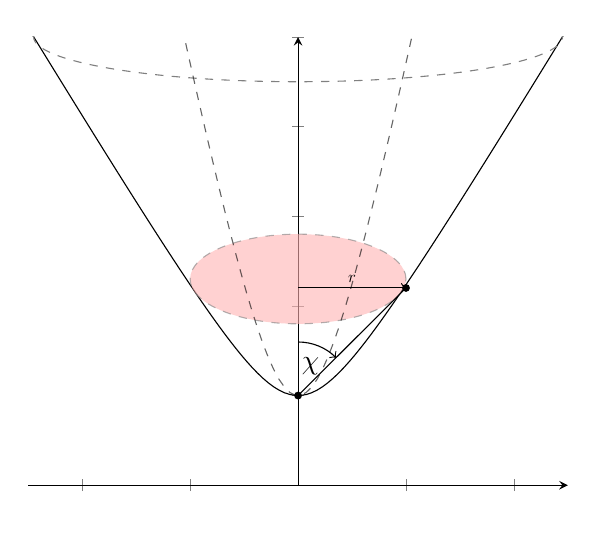
\begin{tikzpicture}
 \begin{axis}[axis lines =center,xmin=-5,xmax=5,ymin=0,ymax=5,xticklabels=false,yticklabels=false]
     \addplot[samples=200,domain=-10:10]{sqrt(1+x^2)};
     \draw[color=gray,dashed, fill=red!30,opacity=0.6] (axis cs: 0,2.3) ellipse (2 and 0.5);
     \draw[color=gray,dashed] (axis cs: 0,5) ellipse (4.9 and 0.5);
      \addplot[samples=200,domain=-10:10,dashed,opacity=0.6]{3*sqrt(1+x^2)-2};
     \draw (0,1) node[circle,fill,inner sep=1] (orig) {};
     \draw (2,2.2) node[circle,fill,inner sep=1] (p) {};
     \addplot[samples=30] coordinates {(0,1)(2,2.2)};
     \draw (0,100) node (y){};
     
     \pic [draw=black,<-,"$\chi$",scale=1.36] {angle = p--orig--y};
     \draw[->](axis cs: 0,2.2)--(axis cs: 2,2.2) node[above,midway,scale=0.6]{$r$};
 \end{axis}

\end{tikzpicture}
\end{document}